There are a variety of tests that can be conducted to verify the performance and
correctness of our  device.  The  following is a list of test fixtures and their
expected results based on simulations.

\subsection{Test Fixtures}

\subsubsection{Trivial VI Curve}


\subsubsection{Non-trivial VI Curve}


\subsubsection{Ripple Voltage and Ripple Current vs Resistive Load}

Using LTspice\cite{ref:ltspice}, the circuit  of  our  regulator was modeled and
the  peak-to-peak  ripple  current  and  voltage  was  simulated using different
resistive  loads ranging from \SI{100}{\milli\ohm} to  \SI{1}{\kilo\ohm}  at  an
output  voltage of \SI{12}{\volt}. Figure \ref{fig:verification:ripple_sim} is a
plot  of  the   ripple   current   and   voltage   versus  the  resistive  load.

\begin{figure}[th!]
    \centering
    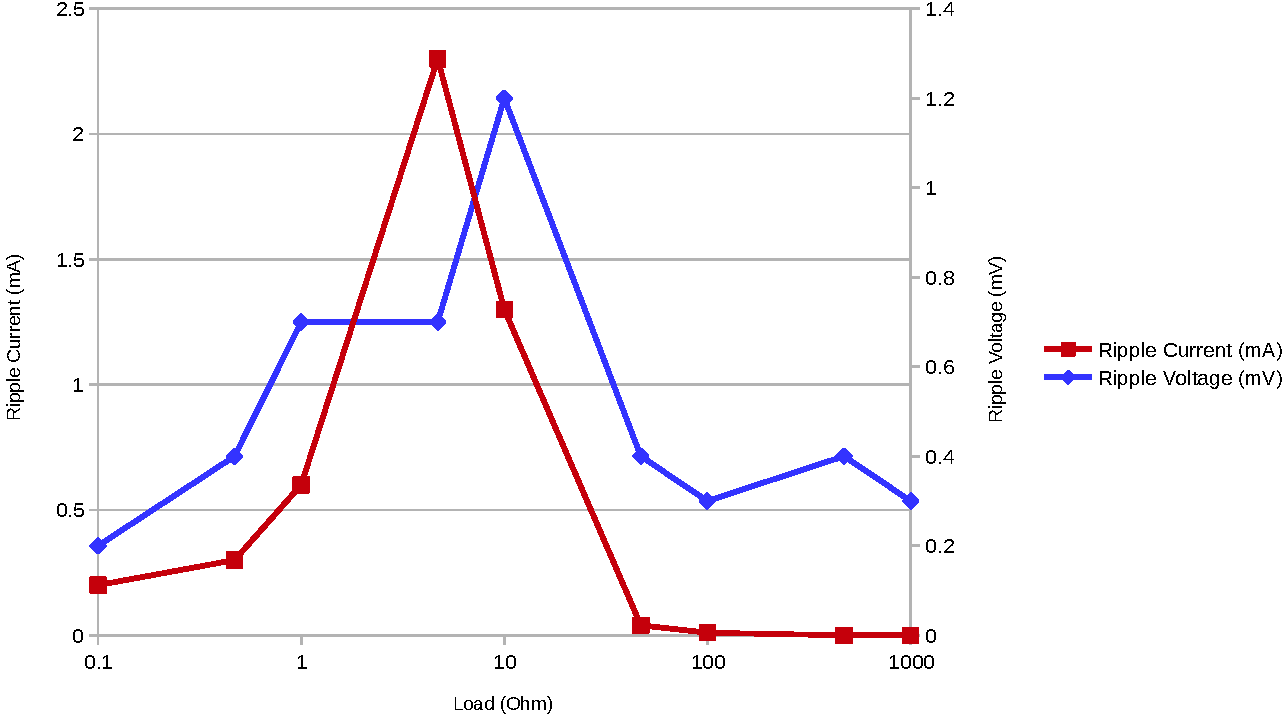
\includegraphics[width=.7\textwidth]{images/sim/ripple-vs-load.pdf}
    \caption{Simulation of the amplitude of the ripple voltage and ripple current vs different resistive loads, obtained using LTspice IV's model of the LT3741}
    \label{fig:verification:ripple_sim}
\end{figure}

In  order  to  test this on the  real  device,  a  constant  output  voltage  of
\SI{12}{\volt} is programmed and a potentiometer  is  attached  to  the device's
output connectors, as illustrated in figure \ref{fig:verification:ripple_fix}

\begin{figure}[th!]
    \centering
    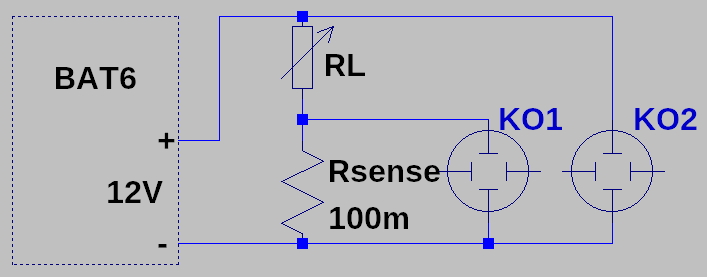
\includegraphics[width=.6\textwidth]{images/sim/ripple-fixture.png}
    \caption{Test fixture for measuring ripple voltage \& ripple current of the device}
    \label{fig:verification:ripple_fix}
\end{figure}

The ripple current  is measured over a small sense resistor $R_{sense}$ using an
oscilloscope. The ripple voltage  is  measured  using  a  second  channel of the
oscilloscope by measuring the output voltage.

The peak-to-peak ripple voltage  and current is measured for different resistive
loads ranging from \SI{100}{\milli\ohm} to \SI{1}{\kilo\ohm} and compared to the
simulated model.


\subsubsection{Power Absorbtion}

As stated in the specifications,  the  device  must  have  the  ability  to sink
current  as  well  as  source  current.  In  order to test this, the  device  is
programmed  to  output  \SI{12}{\volt} and is connected in series with a current
limiting resistor  and  a  second  power  source  set  to  a  higher voltage, as
illustrated      in      figure     \ref{fig:verification:power_absorbtion_fix}.

\begin{figure}[th!]
    \centering
    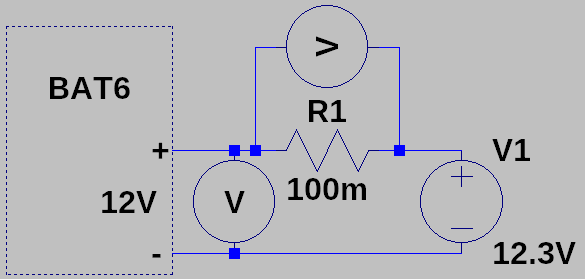
\includegraphics[width=.6\textwidth]{images/sim/power-absorbtion-fixture.png}
    \caption{Test fixture for measuring power absorbtion of the device.}
    \label{fig:verification:power_absorbtion_fix}
\end{figure}

The second voltage source is slowly increased until \SI{3}{\ampere} are  flowing
through  the  current  limiting  resistor  $R_1$  (which  can  be determined  by
measuring the voltage over said resistor), all while the device's output voltage
is closely monitored. The output voltage is expected to remain constant.


\subsubsection{Transient Response}

This test is used  to  determine  the reaction speed of the regulator and the VI
control algorithm when switching  quickly  between  two extreme resistive loads.
The device is programmed to mimic  the  behaviour of a simple solar panel model.
As illustrated in figure \ref{fig:verification:transient_fix} the output voltage
is  measured  using  an oscilloscope and various resistive loads are switched on
and off over the output using a MOSFET and a signal generator.

\begin{figure}[th!]
    \centering
    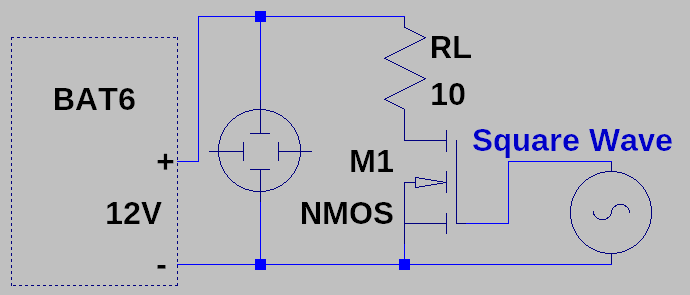
\includegraphics[width=.6\textwidth]{images/sim/transient-fixture.png}
    \caption{Test fixture for measuring the transient response of the device}
    \label{fig:verification:transient_fix}
\end{figure}

The frequency of the signal generator is set  to  a  low  value  such  that  the
device's output voltage is always stable before the load is changed.

The results of this measurement will make a statement over the propagation delay
of  the  algorithm as well as the time it takes for  the  voltage  to  stabilise
again.


\subsubsection{Reactive Loads}

In the course specification we  opted to test the device with various capacitive
and  inductive  loads  out  of  curiosity. During the course of the  project  we
learned that this is not an applicable test because reactive loads are primarily
used for testing the behaviour of power factor correction -- which, according to
the EN61000-3-2  regulations\cite{ref:pfc},  affect  devices consuming more than
\SI{75}{\watt},  meaning  that  the main power supply we use already implements
power factor correction and testing for this would  be meaningless. Furthermore,
the measurements we obtain  from  tests  using  reactive  loads would require an
immense  amount of additional research on our part before the results  could  be
interpreted in any  meaningful way. For this reason we have decided to omit this
test case.


\subsection{Measurement Results}

Unfortunately, we were unable to  operate the LT3741 for a period long enough to
conduct any of the measurements listed above.  The same regulator model (LT3741)
was  permanently  damaged  twice  in  a row. Please see the next section  for  a
detailed analysis on what we think the issue is and how we would proceed if more
time to do so were available.


\subsection{Analysis of the Issue}

\subsubsection{A Quick Overview}

The  first regulator output the correct voltage  of  \SI{12}{\volt}  when  being
supplied  with  \SI{32}{\volt}.  Unplugging the device and re-plugging it into a
\SI{36}{\volt}  power  supply  instantly  damaged  it  permanently.  After  some
detailed measurements it  was  concluded  that  the  high-side driver inside the
LT3741  was somehow damaged and not operating as it should. Our  assumption  was
that -- since we were  operating  the device very closely to its maximum ratings
of  \SI{40}{\volt} -- during switching, the high-side MOSFET driver was  exposed
to transients exceeding the device's absolute maximum ratings  and thus damaging
the driver permanently.

The regulator was replaced with a new  one  and  the  supply voltage was lowered
from  \SI{36}{\volt}  to \SI{28}{\volt} in order to give  more  leeway  for  the
supposed transient voltages. The new regulator appeared  to  output  the correct
voltage of \SI{12}{\volt}, so a resistive load of \SI{80}{\ohm} was connected on
the  output  of  the  regulator.  After  about  \SI{20}{\second}  of  continuous
operation, the output  voltage  again  dropped  and  the  device was permanently
damaged. Unfortunately, we were unable to capture some vital measurements of the
transients we were looking for to confirm our suspicions from the first failure.
It is clear, however, that the damage was not caused by  the device overheating,
as none of the components were remotely warm  to  the touch. This seems to align
with the transient theory.


\subsection{Simulating the Issue}

The physical layout of  the  regulator  and  the  MOSFETs  is depicted in figure
\ref{fig:verification:long_traces_pcb}.  The  physical   length  of  the  traces
connecting the  Switch  (SW),  High  Gate  (HG)  and  Low  Gate (LG) pins of the
regulator to the switching MOSFETs is fairly  long (>\SI{2}{\centi\metre}). Most
of the time, the parasitic  inductances and capacitances are negligible. In this
case, however, they aren't.

The series  inductance  and  series  resistance  is  calculated using an on-line
calculator\cite{ref:trace_inductance}\cite{ref:trace_resistance}   (the   width,
length,    and    thickness    is    known   to    be    \SI{0.4}{\milli\metre},
\SI{2}{\centi\metre}  and \SI{35}{\micro\metre} respectively) and added  to  the
simulation   model  seen  in  figure   \ref{fig:verification:long_traces_model}.


\begin{figure}[th!]
    \centering
    \begin{minipage}{.6\textwidth}
        \centering
        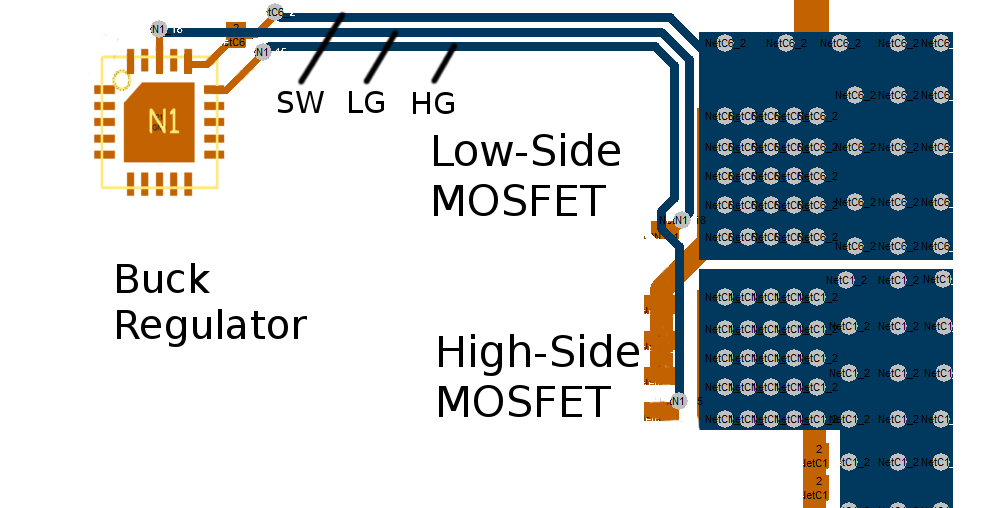
\includegraphics[width=.9\textwidth]{images/pcb/long_traces.png}
        \caption{}
        \label{fig:verification:long_traces_pcb}
    \end{minipage}
    \begin{minipage}{.38\textwidth}
        \centering
        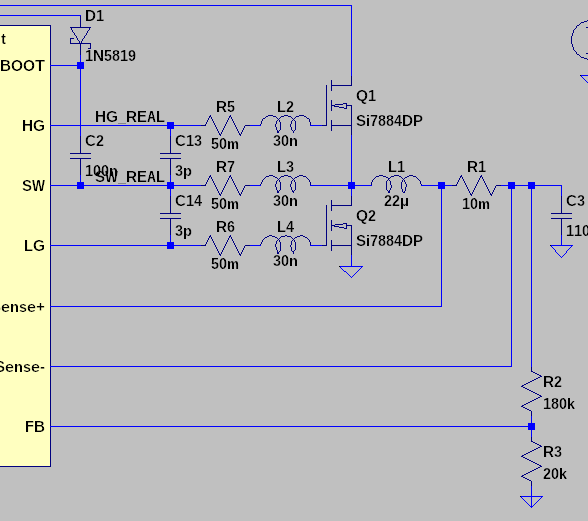
\includegraphics[width=.9\textwidth]{images/sim/lt3741_transients_circuit_real.png}
        \caption{}
        \label{fig:verification:long_traces_model}
    \end{minipage}
\end{figure}

